%!TEX root=../main.tex
\chapter{Methodology}
\label{chap:methology}
\acresetall %reset abbrevations
%\todo{Anything that is related to how the experiments work should be moved. Anything related to the methods themselves (not related to experiments) should stay.}
%\me{4.1 and 4.2 are background, but you advised 1 lvl up. still feels out of place here}
%\todo{ Chapter 4 has a lot of content that belongs to Chapter 5, so I will read it when the content is moved in place. }
%\sug{guide: This section contains the methods used in this thesis. For example, details about the models and adversarial attacks.s}

 
In this chapter, we detail the methodological approach used to model vessel trajectories. We use Section \ref{sec:seq2seq} to establish the theoretical background required for sequence-to-sequence modelling and Section \ref{sec:automl} for the principles of \ac{AutoML}. In the subsequent sections \ref{sec:kinematicimplementation} to \ref{sec:sequenceimplementation}, we describe the exact definitions, state representations, and architectural configurations of the implemented models.
\ws{refer to sections explicitly using the ref command. First, you need to give them labels using label command.} 

\section{Sequence-to-Sequence Models}
\label{sec:seq2seq}
    %https://arxiv.org/html/2406.02770v1#bib.bib14

In the domain of Deep Learning, \acf{Seq2Seq}  Models \ws{they are usually called Seq2Seq, not S2S please modify} 
serve as a \ws{what does dependent sequences mean, elaborate} \me{rephrased, elaborated}
framework for tasks where both input and output take the form of ordered sequences, and the output sequence is conditioned on the input sequence as a whole. That is, each element of the output is not generated independently, but rather informed by the full context of the input (or previously generated outputs).
While \ac{Seq2Seq} is rooted in language processing tasks like translation \parencite{sutskever2014sequencesequencelearningneural}, it can be %dieses zitat vlt raus
applied to any kind of sequential data, ranging from numerical time series and sensor data to genomes and handwriting \parencite{gentleschmidt2019recurrentneuralnetworksrnns}. 
Most \ac{Seq2Seq} models are based on an Encoder-Decoder architecture. 
\ws{`Follow' an architecture is a rather strange expression. Models have architectures, they do not follow them.}
The Encoder processes the input sequence and compresses the information into a fixed-size context vector, typically called \ws{typically called}
the hidden state.
The Decoder uses this vector to generate the output sequence.
Often, this regeneration is implemented autoregressively, meaning only one time step \ws{time step}
is predicted at a time, multiple times in a row with a shifting context window.
\ws{Transition needed to the types of Seq2Seq models}
To implement the encoder and decoder components within this \ac{Seq2Seq} framework, an underlying architecture capable of processing ordered temporal data is required.

    \begin{comment} % zu ausführlich
        
    \begin{itemize}
        \item \textbf{Encoder}: Processes the input sequence and compresses the information into a fixed-size context vector (hidden state).
        \item \textbf{Decoder}: Uses this vector to generate the output sequence (e.g., the predicted GPS positions for the next 10 time steps).
    \end{itemize}
        \end{comment}

    %A graphical overview of Encoder Decoder Sequence Models using the following buidling blocks can be found in Figures \ref{fig:s2s_rnn_appendix}, \ref{fig:s2s_lstm_appendix}, \ref{fig:s2s_bilstm_appendix}, and \ref{fig:s2s_attention_appendix}:

    %Encoder and Decoder can for example be built with the following two building blocks:%bessere überleitung todo

    
\ws{Please convert these to paragraphs instead of subsections (or just in-line text) for both RNN and LSTM, and make them briefer. No need to get into the technical details of RNNs and LSTMs to this extent. You can write a brief version in the main paper and move the details to the appendix} 
\paragraph{RNNs and LSTMs.}
The core architecture for sequence-based learning is the \ac{RNN}.
The primary distinction between \acp{RNN} and conventional Feedforward Neural Networks is the direction of information flow.
Instead of a strictly forward pass, an \ac{RNN} utilises cycles to feed information back into the hidden state, which enables the incorporation of context from previous inputs.
As the sequence length increases, standard \acp{RNN} suffer from the vanishing gradient problem, which limits their capability to learn long-term dependencies.
To address this limitation, the \ac{LSTM} architecture was introduced.
The core innovation of the \ac{LSTM} is a cell state regulated by three gates. The forget, input, and output gates allow relevant information to persist across many time steps.
Furthermore, the architecture is mathematically equipped for multivariate sequence modelling. This allows the representation of non linear cross-channel correlations.
When implementing \acp{LSTM} within \ac{Seq2Seq} frameworks, several architectural configurations must be considered. 
Key design parameters include the number and direction of the hidden layers, as well as the choice of decoding strategy, which typically involves either a direct linear mapping or an autoregressive approach.
A more detailed mathematical description of the internal update processes for both \acp{RNN} and \acp{LSTM}, along with illustrations of the architectures can be found in Appendix \ref{appx: mathfoundations}.

   
    

    \begin{comment} % leider garnicht benutzt außer in related work, was diese mkapitel vorausgeht. wenn platz habe kann man wieder reinpacken
        
    \subsubsection{Bi-LSTM}
    Many variants and extensions of the \ac{LSTM} have been proposed to enhance its representative power. A notable architectural advancement is the \ac{Bi-LSTM}. While \cite{sutskever2014sequencesequencelearningneural} demonstrated that simply reversing the input sequence in a unidirectional \ac{Seq2Seq} model can significantly improve performance, the \ac{Bi-LSTM}, first introduced by \cite{articlebilstmorigins} formalizes this concept in its architecture .
    
    A \ac{Bi-LSTM} consists of two parallel hidden layers: a \textit{forward \ac{LSTM}} that processes the sequence in chronological order and a \textit{backward \ac{LSTM}} that processes it in reverse. Their respective hidden state outputs are then concatenated, added, averaged or multiplied  to form the final output. 
    Recent studies, such as \cite{articlebilstmsus} claim this makes the \ac{Bi-LSTM} more suitable for vessel trajectory prediction. 
   
    However, the application of \acp{Bi-LSTM} in autonomous systems and \ac{MTT} requires us to consider causality. Because the backward pass requires knowledge of the entire sequence up to the final time step, \acp{Bi-LSTM} are non-causal. Consequently, they cannot be used within the decoder of our \ac{Seq2Seq} Model. Nevertheless, they can be applied within the encoder stage. This allows the model to generate a richer input vector, which is then processed by a unidirectional decoder to predict future motion. %blabla als  hyperparameter in optimierer.. evtl auch schon hier den teil in methologie schreiben, mit tim klörne

      % 7 zusammenfassung: xlstm besser skalierbar, größerer speicher. aber für unsere 10 timesteps overkill. außerdem größerer feature space, schwerer (Schnell) manuell zu tunen, was unsere vorteile wettmachen würde + mangelnde vergeichbarkeit weil neu, . also nur kurz erklären
    %xlstm liefert die grundlage für ein lstm basiertes foundation modell durch erweiterung mit ..., aber dieses exisistiert leider noch nicht. wenn ich den platz habe würde ich gerne
    \end{comment}

    \paragraph{x-LSTM.} 
    \ws{please be consistent with . after the text in the paragraph. It is missing here and in other places in the thesis. Please check}
    Many variants and extensions of the \ac{LSTM} have been proposed.
    Recently, \textcite{beck2024xlstmextendedlongshortterm} introduced the \ac{x-LSTM} architecture to address bottlenecks of \ac{LSTM}. The primary goals of this architecture are to improve hardware scalability and to provide a larger memory capacity. To achieve this, two new \ac{LSTM} Layers are introduced:
    
    \begin{itemize}
        \item \textbf{\ac{s-LSTM}}: introduces exponential gating, which allows the model to revise and update its memory more dynamically.
        \item \textbf{\ac{m-LSTM}}: replaces the traditional vector cell state and its element-wise updates with a matrix memory updated via matrix multiplication. This %structural shift eliminates the sequential dependency of the hidden state, enabling 
        enables fully parallelised sequence processing during training.
    \end{itemize}
    Using these layers, an \ac{x-LSTM} can maintain the linear time complexity $\mathcal{O}(N)$ of conventional \acp{RNN} during inference, in contrast to the quadratic complexity of Transformers. \parencite{beck2024xlstmextendedlongshortterm, attentioniayn} %for respective Time omplexity 
    
    %However, the application of \ac{x-LSTM} in this work introduces practical challenges. 
    For our specific use case of predicting short 10-step trajectories, the expanded memory capacity offers limited benefits while introducing computational overhead. Furthermore, the architecture requires additional hyperparameters, such as the choice between \ac{s-LSTM} and \ac{m-LSTM} layers, as well as matrix dimensions. %number of heads.. aber die will ich hier nicht einführen
    This expands the search space for \ac{HPO} substantially.%, makes the tuning process computationally more expensive and harder to balance against simpler models. %Finally, as a recently proposed architecture, utilizing \ac{x-LSTM} would limit the comparability of our results with existing \ac{LSTM}-based maritime tracking approaches. 
    
    Nevertheless, because of it's scaling capabilities, the \ac{x-LSTM} builds the basis of the TiRex foundation model (Section \ref{subsec:foundation}).

\ws{The following can also be paragraphs instead of subsections}

\paragraph{Attention and Transformers.}
%ziemlcih kurz davor dass es sota ist, aber für uns ist hier alles gesagt, oder?
\ac{Seq2Seq} architectures based on \acp{RNN} or \acp{LSTM} face a structural limitation: The encoder must compress the entire input sequence into a single, fixed-size context vector. %, and information is lost. 
This compression creates an information bottleneck, causing the network to forget earlier parts of the sequence as the input length increases.  
\ws{This phrasing is not accurate. Now, you are claiming that because of compression, all `information' is lost. Also, the attention mechanism solved the `forgetting' problem rather than `lost' information. Please rephrase.} \me{added bottleneck}
To resolve this forgetting problem, \textcite{bahdanau2016neuralmachinetranslationjointly} introduced the attention mechanism.
Instead of relying on the final hidden state, attention allows the decoder to access all intermediate hidden states of the encoder. At each decoding step, the mechanism calculates an alignment score, which enables the model to assign higher weights to the timestamps most relevant to the current prediction.
Building upon this, \textcite{attentioniayn} proposed the Transformer architecture, which completely discards recurrent layers (such as \ac{RNN} or \ac{LSTM}) in favor of Self-Attention. 
Self-Attention computes the relational importance of all data points within a sequence simultaneously. This enables the models \ws{it does not allow `us'. We do not capture anything, the model does. Please rephrase}
to capture global dependencies.
%noch bischen umformulieren. filler weg un abschwächen evtl
However, applying Transformers to %short physical 
time series, such as our \ac{AIS} trajectories, presents new challenges. Unlike \acp{LSTM}, Transformers lack an inductive bias for sequential order and must rely on artificial positional encoding. 
A %recent 
critique by % in time series research 
\textcite{zeng2022transformerseffectivetimeseries} suggests that for short, physically continuous sequences where simple local dependencies dominate, Transformers can be unnecessarily complex, computationally expensive, and prone to overfitting compared to recurrent or linear models.
\ws{The citation should come at the end of the claim} \me{i resolved this by using singular with textcite.  i wanted to avoid making this sound like the source is a survey}.
Nonetheless, their capacity to parallelise efficiently has popularised Transformers as an architecture in large-scale predictive modelling. %needs citation ?
%\todo{factcheck skalierung}

\paragraph{Foundation Models.}
\label{subsec:foundation}
Because Transformers parallelise so effectively, they enabled the creation of Foundation Models. These are massive neural networks pretrained on vast, diverse datasets, across multiple domains such as weather, finance, and sensor data, to learn universal sequence patterns before being applied to a specific task. After being trained on very general data, they can be fine-tuned or adapted to specific tasks with relatively small amounts of task-specific data \parencite{Liang_2024foundation}.

A prominent example in time series forecasting is \textbf{Chronos} \parencite{ansari2024chronoslearninglanguagetime}, which tokenises time series values and processes them using a pure encoder architecture, or the more recent adaption \textbf{Chronos-2} \parencite{ansari2025chronos2}, which uses group attention to maintain weights across channels and enable multivariate or covariate informed forecasting. For our vessel trajectory prediction, Foundation Models offer two  application paradigms:
\begin{itemize}
    \item \textbf{Zero-Shot Forecasting:} The pretrained model generates predictions for \ac{AIS} trajectories without ever having been trained on maritime data. Chronos in particular was developed to  have comparable and occasionally superior zero-shot performance on new datasets, relative to methods that were trained specifically on them \parencite{ansari2024chronoslearninglanguagetime}.
    \item \textbf{Fine-Tuning (Warm Starting):} The model is can be trained on our specific domain data. By initialising \ws{british english}
    the training process with pretrained weights (a \enquote{warm start}) rather than random initialisation, the model requires significantly less domain data and computational time to adapt to the specific kinematics of inland vessels. %\me{we dont do that. still include the possibility?}
\end{itemize}% \me{only did zero shot, shorten?}

%While Transformer based foundation models represent the current state-of-the-art in generalized forecasting, they come with computational overhead. %wieso habe ich das geschreiben, das ist ja nur inferenz

The \ac{x-LSTM} architecture \parencite{beck2024xlstmextendedlongshortterm} addresses the  \ws{cannot use possesive s with inanimate} 
lack of sequential bias of the Transformer while maintaining extreme scalability. %O(N) in lstm anzahl layer vs O(n^2) für Transformer as mentioned before
Consequently, \acp{x-LSTM} provide the theoretical basis for \ac{RNN}-based Foundation Models. 
The \textbf{TiRex} foundation model,
%One very recent foundation model, \textbf{TiRex},
\ws{no need to mention very recent. These expressions are reserved to `related work'} 
 which leverages the \ac{x-LSTM}, was presented by \textcite{auer2025tirexzeroshotforecastinglongtrex} and showed promising results in benchmarks against Chronos. However, the authors have noted the model does not perform well with multivariate times eries data. As a consequence, applicability to \ac{AIS} Trajectories is limited \ws{is limited ... then give reasons.}
, because the univariate model treats individual features as independent channels, which prevents it from capturing cross-correlations. Since vessel dynamics are governed by physical constraints where \ac{SOG} and \ac{COG} directly impact the trajectory, this approach may result in kinematically inconsistent predictions.

\ws{Never use future tense for completed work. The future tense is only use when you write a plan}    
We will benchmarked our self-trained \ac{LSTM} model against Chronos-2 and TiRex to both investigate whether generalised, pretrained knowledge outweighs physically grounded, domain-specific recurrence, and test zero shot performance of \ac{x-LSTM} based foundation model vs Transformer based.
    

\section{Automated Machine Learning}
%todo some rephrasing, more details on hyperband, explain cash similar level to hpo

\label{sec:automl}

The development of machine learning applications traditionally relies on human intervention and domain expertise.
\ac{AutoML} aims to reduce the manual effort and knowledge required by automating design choices.
These choices include decisions regarding model architecture, evaluation, and optimisation \parencite{hutter2019automated}.
The primary goal of \ac{AutoML} is to make machine learning accessible to non-experts, while also accelerating the development process for experienced ML-engineers by removing repetitive tasks \parencite{AutoMLHoos, hutter2019automated}.
The automated configuration of a machine learning model is fundamentally defined by three core components.
First, a search space must be established to set the boundaries of all permissible model configurations.
Second, a search strategy is required to systematically navigate this multidimensional space and identify promising candidates.
Finally, we need to define performance estimation methods to evaluate the sampled configurations.
In this work, \ac{AutoML} is utilised specifically for \ac{HPO}, as detailed in Section \ref{subsec:automlhpo}.s
 The concepts of search spaces and search strategies are covered in the following subsections \ref{subsec:search_space} and \ref{subsec:searchstrat}. The methodology for performance evaluation is addressed separately within Chapter \ref{chap:experimentalsetup}.
\ws{Too many details in this secion as well. You can mention briefly the methods you used and move the deep details to the appendix. Examples, no need to explain how BO works in the main thesis content.}
\ws{No transition here. You mentioned steps then jumped to something called `the search space'. You need a transition here. Example, remove the steps and mention the components of AutoML instead, then explain them one by one in subchapters (as it is now)}. \me{did a rewrite of this section. content moved to appendix and chatper 5, intro and transitions adjusted}

\subsection{The Search Space}
\label{subsec:search_space}

The foundation of any \ac{AutoML} problem is the definition of its search space. WIth the search space, we set the boundaries of the automated system and define the set of all possible configurations that the optimiser is allowed to explore to find the configuration with the best performance.

\paragraph{Hyperparameter Optimisation.}
\label{subsubsection:HPO}
Hyperparameters control the learning process of a model, but they cannot be derived from training data via standard gradient-based optimisation.
As a result, they must be set prior to training \parencite{hutter2019automated}.
In \ac{HPO}, the search space is restricted to the hyperparameters of a single, predefined learning algorithm.
These parameters can be continuous, integer-valued, or categorical.

\paragraph{Model Selection.}
Model selection is applied at a higher level of abstraction than \ac{HPO}.
Instead of tuning the internal mechanics of a specific algorithm, the search space consists of a discrete set of different machine learning algorithms to identify the algorithm family that best models the underlying data distribution.




\paragraph{CASH Problem.}
In practice, model selection and \ac{HPO} are intertwined, because the optimal hyperparameters depend entirely on the chosen algorithm.
This interdependency is formulated as the \ac{CASH} problem.
When formulating \ac{CASH} as a single, joint optimisation problem, the search space grows exponentially.
The combination of discrete algorithm choices with their respective continuous, discrete, and categorical hyperparameters presents a massive computational challenge.
Consequently, solving the \ac{CASH} problem efficiently typically requires meta-learning or a warm start, where metadata and historical performance records from previously evaluated datasets are utilised \parencite{AutoMLHoos}.
Because such extensive metadata is not available for the specific inland vessel trajectories utilised in this work, addressing the full \ac{CASH} problem is computationally unfeasible.
A detailed mathematical formalisation of \ac{HPO}, model selection, and the \ac{CASH} problem is provided in Appendix \ref{app:math_search_space}.

\paragraph{NAS Problem.} \me{can i delete this paragraph? only mentioned here to give a full picture of automl)}
\acf{NAS} expands the search space even further by fully automating the design of the neural network architecture itself. Instead of selecting predefined algorithms, \ac{NAS} optimises the arrangement of operations, layer connectivity, and network depth \parencite{AutoMLHoos}. Due to the immense size of the resulting search space, \ac{NAS} requires unfeasable computational resources and falls out of scope for this thesis. In practice, \ac{NAS} is typically only applied once the fundamental type of layer (e.g., \ac{LSTM} or Transformer) has already been established.


\begin{comment} %sompressed and moved details to appendix
    
The development of machine learning applications traditionally relies on human intervention and domain expertise. \ac{AutoML} aims to reduce the manual effort and knowledge required by automating design choices. Those choices include decisions regarding model architecture, evaluation, and optimisation \parencite{hutter2019automated}. The primary goal of \ac{AutoML} is to make machine learning accessible to non-experts, while also accelerating the development process for experienced ML-engineers by removing repetitive tasks \parencite{AutoMLHoos, hutter2019automated}.

Analogous \ws{do you mean analogous?} \me{yes :)}
to the traditional pipeline, a complete \ac{AutoML} pipeline can be broadly categorised into the following stages:
\begin{itemize}
    \item \textbf{Data Preparation and Feature Engineering:} Automatically cleaning raw data, imputing missing values, and constructing or selecting relevant features.
    \item \textbf{Model Selection:} Choosing the appropriate mathematical model or algorithm family for the given dataset.
    \item \textbf{\ac{HPO}:} Tuning the configuration parameters that control the learning process of a selected model.
\end{itemize}
\ws{This sentece is out of place}
In this work, \ac{AutoML} was used for \ac{HPO}, as detailed in Section \ref{subsec:automlhpo}. 
\ws{until here} \me{put back below the enumeration. this takes up more space unfortunately}
%In this work, \ac{AutoML} was used for \ac{HPO}, as detailed in Section \ref{subsec:automlhpo}. spart mir eine zeile

\ws{No transition here. You mentioned steps then jumped to something called `the search space'. You need a transition here. Example, remove the steps and mention the components of AutoML instead, then explain them one by one in subchapters (as it is now)}.
\subsection{The Search Space}
\ws{use title case in the titles} \me{applied everywhere}
The foundation of any \ac{AutoML} problem is the definition of its search space. This space sets the boundaries of the automated system and defines the set of all possible configurations that the optimiser is allowed to explore to find the configuration with the best performance.

\paragraph{Hyperparameter Optimisation.}
\label{subsubsection:HPO}

Hyperparameters control the learning process of a model but, unlike model parameters (weights), cannot be derived from training data via standard gradient-based optimisation. As a result, we need to set them prior to training \parencite{hutter2019automated}. \ac{HPO} restricts the search space to the hyperparameters of a single, predefined learning algorithm.

\ws{Too many details in this secion as well. You can mention briefly the methods you used and move the deep details to the appendix. Examples, no need to explain how BO works in the main thesis content.}
\me{überlegen was alles ins appendix kann und wie ich das dann strukturiere. BO ist schon weg. next: 4.2.1 mathe in anhang4.5.2 in experiment teilweise. rest nur auf nachfrage}

Formally, adapted from \textcite{AutoMLHoos} to reflect the fixed training and validation split we use, we can let $A_\lambda$ denote a learning algorithm $A$ instantiated with hyperparameter configuration $\lambda \in \Lambda$, where $\Lambda$ is the
hyperparameter search space. Given a dataset $\mathcal{D}$ split into a training set $\mathcal{D}_\text{train}$ and a validation set
$\mathcal{D}_\text{val}$, the \ac{HPO} objective is:
\begin{equation*}
    \lambda^* = \underset{\lambda \in \Lambda}{\arg\min}\;
    \mathcal{L}\!\left(A_\lambda,\, \mathcal{D}_\text{train},\,
    \mathcal{D}_\text{val}\right)
    \label{eq:hpo}
\end{equation*}
where $\mathcal{L}$ is a validation loss metric. Since evaluating $\mathcal{L}$ requires fully training $A_\lambda$, each function evaluation is expensive, and \ac{HPO} is a black-box optimisation problem.

Hyperparameters can be of several types, which together determine the structure of $\Lambda$, such as:
\begin{itemize}
    \item \textbf{Continuous:} Real-valued parameters such as the learning
    rate or regularisation strength. They are typically searched on a
    log-uniform scale.
    \item \textbf{Integer-valued:} Discrete but ordered parameters, such as
    the number of hidden units or the sequence input length.
    \item \textbf{Categorical:} Unordered discrete choices, such as the
    type of optimiser, the activation function or the set of input features.
    %\item \textbf{Conditional:} Parameters that are only relevant given a
    %specific value of another hyperparameter. For example, the dropout rate
    %is only meaningful if a dropout layer is included in the architecture.
    %Conditional hyperparameters introduce a hierarchical structure into
    %$\Lambda$, commonly represented as a \emph{configuration space}
    %\parencite{hutter2019automated}.
\end{itemize}





\paragraph{Model Selection.}
Model Selection operates at a higher level of abstraction than \ac{HPO}. Instead of tuning the internal mechanics of a specific algorithm, the search space consists of a discrete set of different machine learning algorithms $\mathcal{A} = \{A^{(1)}, \dots, A^{(R)}\}$ (e.g., \ac{LSTM} vs. Transformer). The objective is to identify the algorithm family that best models the underlying data distribution. 


Formally, adapted from \textcite{AutoMLHoos} to reflect the fixed training and validation split we use%rather than $k$-fold cross-validation
, the algorithm selection problem can be defined as finding the algorithm $A^* \in \mathcal{A}$ that yields the best performance on the validation set:
\begin{equation*}
    A^* = \underset{A \in \mathcal{A}}{\arg\min}\;
    \mathcal{L}\!\left(A,\, \mathcal{D}_\text{train},\,
    \mathcal{D}_\text{val}\right)
    \label{eq:model_selection}
\end{equation*}
%Because one of our deliverables is a model comparison, Model selection is not used for the thesis, as in a \ac{CASH} Problem, not every model is evaluated at it's full capability. das war mir nicht präzise genug. müsste man genau reindiven aber ist auch irrelevant wenn keiner danach fragt

\paragraph{CASH Problem.}
In practice, Model Selection and \ac{HPO} are intertwined: the optimal hyperparameters depend entirely on the chosen algorithm, and the true potential of an algorithm can only be evaluated if its hyperparameters are properly tuned. \textcite{hutter2019automated} formulate this interdependency as the \acf{CASH} problem.%: Combined Algorithm Selection and Hyperparameter optimisation. 

Formally, again adapted from \textcite{AutoMLHoos} to reflect the fixed training and validation split, given a set of learning algorithms $\mathcal{A}$, where each algorithm $A^{(j)} \in \mathcal{A}$ has an associated hyperparameter configuration space $\Lambda^{(j)}$, the \ac{CASH} problem seeks to jointly find the optimal algorithm $A^*$ and its optimal hyperparameter configuration $\lambda^*$:% \parencite{AutoMLHoos}:
\begin{equation*}
    A^*, \lambda^* = \underset{A^{(j)} \in \mathcal{A},\, \lambda \in \Lambda^{(j)}}{\arg\min}\;
    \mathcal{L}\!\left(A^{(j)}_\lambda,\, \mathcal{D}_\text{train},\,
    \mathcal{D}_\text{val}\right)
    \label{eq:cash}
\end{equation*}

When formulating \ac{CASH} as a single, joint optimisation problem, the search space grows exponentially. Combining the discrete choices of algorithms with their respective continuous, discrete, and categorical hyperparameters creates a massive computational challenge. Typically, solving the \ac{CASH} problem efficiently requires meta-learning or a \emph{warm start}, which uses metadata and historical performance records from previously evaluated datasets \parencite{AutoMLHoos}. Because such extensive metadata is not available for the specific inland vessel trajectories utilised in this work, addressing the full \ac{CASH} problem is computationally unfeasible for this thesis. %in methologie?


\paragraph{NAS Problem.} \me{can i delete this? only mentioned here to give a full picture of automl)}
\acf{NAS} expands the search space even further by fully automating the design of the neural network architecture itself. Instead of selecting predefined algorithms, \ac{NAS} optimises the arrangement of operations, layer connectivity, and network depth \parencite{AutoMLHoos}. Due to the immense size of the resulting search space, \ac{NAS} requires unfeasable computational resources and falls out of scope for this thesis. In practice, \ac{NAS} is typically only applied once the fundamental type of layer (e.g., \ac{LSTM} or Transformer) has already been established.

\end{comment}
\subsection{Search Strategies and Pruning}
\label{subsec:searchstrat}
Once a search space is defined, the \ac{AutoML} system requires a strategy to navigate it. Standard search strategies include Grid Search, which evaluates all predefined combinations, and Random Search, which samples configurations uniformly at random. While Random Search is generally more efficient in high-dimensional spaces, %whose performance function has low effective dimensionality
both methods are uninformed and do not utilise past evaluations to guide future selections \parencite{hutter2019automated}. Advanced, informed strategies, such as \acf{BO} , build a probabilistic surrogate model of the objective function to sample only the most promising regions of the search space. %kept this the same
%As an informed search strategy, \ac{BO} builds a probabilistic surrogate model of the objective function to predict the performance of unseen hyperparameter configurations.
Traditional \ac{BO} approaches relying on Gaussian Processes model the probability of the objective value given the hyperparameters directly \parencite{hutter2019automated}.
This direct approach becomes computationally expensive as the number of evaluations grows and scales poorly in high-dimensional configuration spaces \parencite{hutter2019automated}. Moreover, Gaussian process based \ac{BO} cannot natively handle mixed hyperparameter spaces and requires approximations to evaluate categorical variables \cite{AutoMLHoos}. 
To address these limitations, we used the \ac{TPE} algorithm \parencite{bergstra2011algorithms} in this work.
Rather than modelling the objective function directly, the \ac{TPE} inverts the process by modelling the probability of the hyperparameters given the objective value, partitioning past observations into sets of good and bad configurations.
This inversion provides a significant advantage for tuning complex sequence models, as the primary strength of the \ac{TPE} lies in its robust handling of discrete and categorical hyperparameters \parencite{AutoMLHoos}.
Furthermore, each iteration of the algorithm scales linearly with the number of hyperparameters.
A more detailed technical description of \ac{BO} and the \ac{TPE} algorithm is provided in Appendix~\ref{appx:BOandTPE}.

Search strategies are frequently paired with pruning mechanisms.
Through pruning, or early stopping, the training of unpromising configurations is terminated before the maximum allocated budget is consumed.
In methods such as Successive Halving, a large number of configurations are evaluated for a few epochs, the worst-performing candidates are discarded, and more computational resources are allocated to the top performers.

% ----------------------------------------------------------------------
\begin{comment} %moved to appendix
    
Once a search space is defined, the \ac{AutoML} system requires a strategy to navigate it. Standard search strategies include Grid Search, which evaluates all predefined combinations, and Random Search, which samples configurations uniformly at random. While Random Search is generally more efficient in high-dimensional spaces, %whose performance function has low effective dimensionality
both methods are uninformed and do not utilise past evaluations to guide future selections \parencite{hutter2019automated}. Advanced, informed strategies, such as \acf{BO} , build a probabilistic surrogate model of the objective function to sample only the most promising regions of the search space. 


\paragraph{Bayesian Optimisation.}
\acf{BO} uses past evaluations to make informed decisions about which hyperparameters to test next \parencite{hutter2019automated}. This is critical for models where evaluating the true objective function $\mathcal{L}$ is computationally expensive (i.e., fully training an \ac{LSTM}). %lstm example not covered by hutteretal

\ac{BO} achieves this by constructing a probabilistic surrogate model $\hat{f}$, which approximates the true, expensive loss function based on all previously evaluated configurations. Because the surrogate model $\hat{f}$ is cheap to evaluate, the optimiser can test more potential configurations internally to identify the most promising candidates before committing resources to a full model training.

To decide which configuration to evaluate next based on the given surrogate model, \ac{BO} relies on an acquisition function. A commonly used acquisition function is \acf{EI} \parencite{AutoMLHoos}. \ac{EI} evaluates a candidate by combining two essential terms: the expected value of the function at a given point, and the associated variance %, or uncertainty %also covered by automlhoos. jsut wanted to assosiate it earlier
. This combination provides a trade-off between two competing goals:
\begin{itemize}
    \item \textbf{Exploitation:} By considering the expected value, the search is focused on promising regions of the search space that contain good candidate solutions with high probability.
    \item \textbf{Exploration:} In contrast, the variance term encourages the exploration of unknown areas that are weakly explored, or where candidate solutions of highly variable quality have been observed \parencite{Jones1998}.%, AutoMLHoos}. \me{Das ist ein Sekundärzitat, nachfragen}
    %\me{I was unsure how to handle citations here. Jones is the original source, found in AutoMLHoos. i read both. we talked about it}
\end{itemize}
Figure~\ref{fig:bo_illustration} illustrates one iteration of this process. %published as open acces. Open access works published by Springer Nature are published under Creative Commons licences.tdoo resolved (check licensing, otherwise use the one from the literature overview automl timeseries)

\begin{figure} [h]
    \centering
    % Adjust trim values (left bottom right top) 
    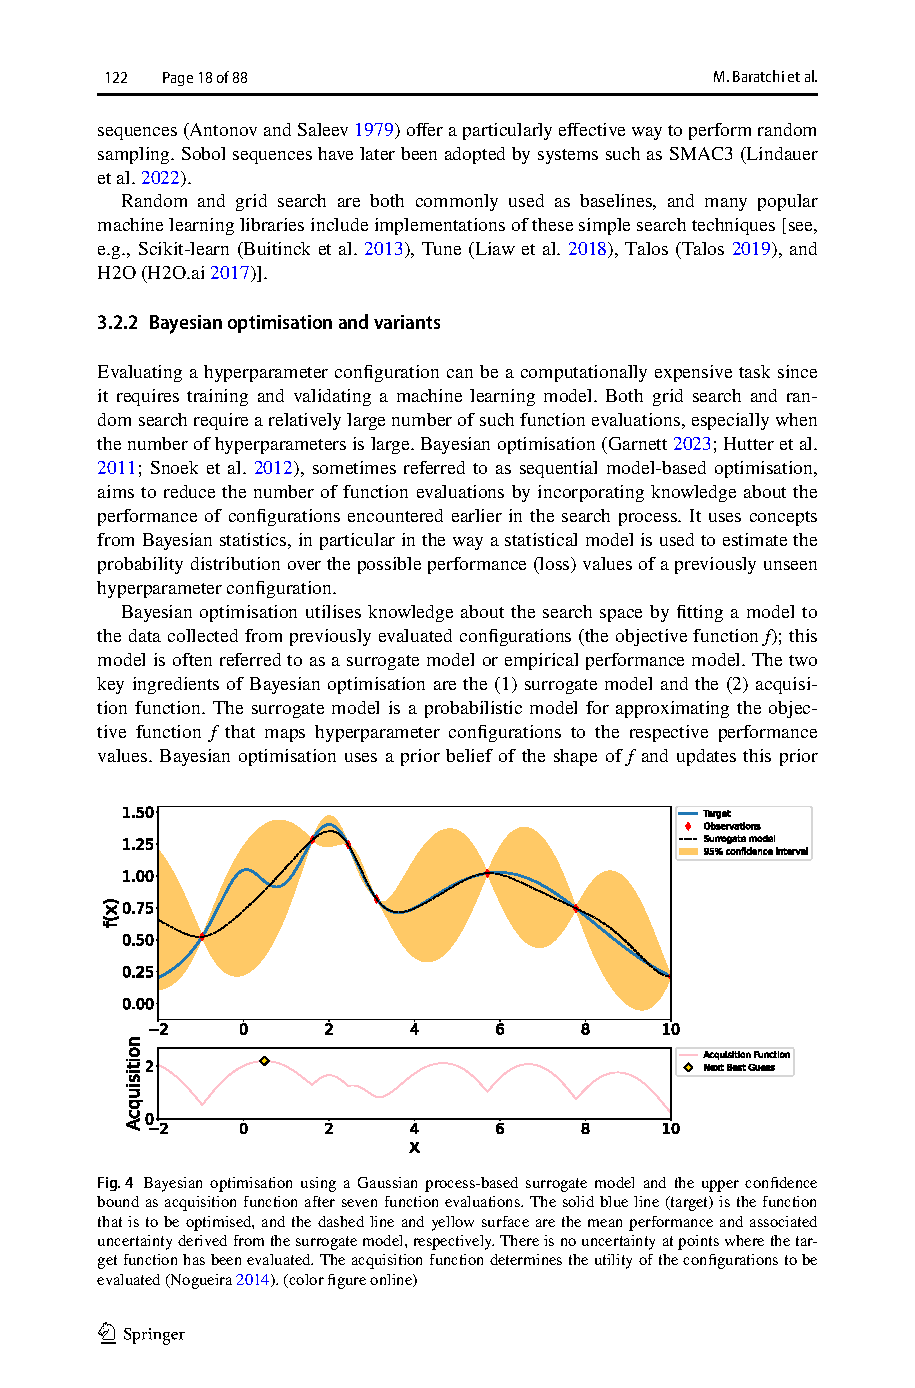
\includegraphics[width=0.8\linewidth,trim={2cm 4cm 2cm 13.5cm}, clip]{figures/985693BO.pdf}
    \caption[Bayesian Optimisation]{\acf{BO} using a surrogate model and \acf{EI} after several evaluations. The solid line represents the true objective $\mathcal{L}$, the dashed line and shaded region show the surrogate mean and 95\% confidence interval, respectively. The acquisition function (bottom) determines the next candidate configuration to evaluate \parencite{AutoMLHoos}.}
    \label{fig:bo_illustration}
\end{figure}

%Common algorithms used as surrogate models include \emph{Gaussian Processes} and \emph{Random Forests}. While Gaussian Processes provide good uncertainty estimates for continuous parameters, Random Forests are often preferred in \ac{AutoML} frameworks such as \ac{SMAC}, because they scale more efficiently and natively handle discrete and categorical hyperparameters \parencite{AutoMLHoos}. \me{maybe delete paragraph, irrelevant. also maybe dont explain Ei if i dont use it, but i think its fine as a baseline}
While classical\ac{BO} surrogate models such as Gaussian Processes model $p(y \mid \lambda)$ directly, they can scale poorly with the number of hyperparameters and struggle with discrete and categorical parameters.

\paragraph{Tree-Structured Parzen Estimator.} 
The \ac{TPE} \parencite{bergstra2011algorithms} addresses these limitations of \ac{BO} by inverting the modelling problem. This enables better handling of categrical hyperparameters. Rather than directly modelling $p(y \mid \lambda)$, the \ac{TPE} instead constructs two separate density functions, $p(\lambda \mid y < \alpha)$ and $p(\lambda \mid y \geq \alpha)$. The threshold $\alpha$ partitions all observations into a set of good and bad configurations, each of which is modeled using one-dimensional Parzen windows. 
Parzen windows are kernel density estimators that place a smooth Gaussian function at each data point, with their sum forming the density function.
 The ratio $\frac{p(\lambda\mid y \ge \alpha)}{p(\lambda\mid y < \alpha)}$ is closely related to the expected improvement acquisition function and serves as the criterion for proposing new hyperparameter configurations \parencite{bergstra2011algorithms, hutter2019automated}. \ac{TPE} further scales linearly with the number of hyperparameters \parencite{AutoMLHoos}. %Through maintaining a sorted list of confgurations in memory, 
\me{ probably replace BO graphic with the TPE figure i made for the defense}

\end{comment}


%%%%%%%%%%%%%%%%%
\ws{Please move the full text to the chapter tex file. This reference is just extra complication with no benefits}

%
%!TEX root=../main.tex
\chapter{Background} %7-10 pages, will be  hard  to do lesss
\label{chap:background}

\section{Trajectory prediction in maritime/AIS}%core SOTA
\section{Motion Models} \todo{fill once I implemented them}
    \subsection{CV}
    %\subsection{CA}
    \subsection{CTRV}
    %\subsection{IMM?} ich denke nicht, darauf  soll der fokusnicht liegen
\section{Sequence-to-Sequence Models}   
    %https://arxiv.org/html/2406.02770v1#bib.bib14

  \todo{graphics in universal style. They do not help me a lot personally, so I did not include them yet}

    In the domain of Deep Learning, \ac{S2S}  Models serve as a framework for tasks where input and output are dependent sequences. While \ac{S2S} is rooted in language processing tasks like translation \cite{sutskever2014sequencesequencelearningneural}, it can be %dieses zitat vlt raus
    applied to any kind of sequential data, ranging from numerical time series and sensor data to genomes and handwriting \cite{gentleschmidt2019recurrentneuralnetworksrnns}. 
    Most \ac{S2S} models follow an \textbf{Encoder-Decoder} architecture. 
    \begin{itemize}
        \item \textbf{Encoder}: Processes the input sequence and compresses the information into a fixed-size context vector (hidden state).
        \item \textbf{Decoder}: Uses this vector to generate the output sequence (e.g., the predicted GPS positions for the next 10 time steps).
    \end{itemize}
    Encoder and Decoder can for example be built with the following two building blocks:%bessere überleitung todo

    \subsection{RNN}
    Building on the first popular model to use recurrence, the Hopfield Network introduced by \cite{hopfieldrnn}, the foundational concept for sequence-based learning is the \ac{RNN}. 
    The primary distinction between \acp{RNN} and conventional Feedforward Neural Networks, such as \acp{MLP}, is the direction of information flow. While Feedforward Networks are acyclic, \acp{RNN} use cycles to feed information back into the hidden state, the \textit{memory}. This architecture allows the model to incorporate historical context from previous inputs $X_{0:t-1}$ when processing the current input $X_t$, rather than treating each input in isolation \cite{gentleschmidt2019recurrentneuralnetworksrnns} and to make decisions based on the patterns it recognizes \cite{AIBook}. The recurrence can be expressed as:

    \begin{equation}
        H_t = \phi_h (X_t W_{xh} + H_{t-1} W_{hh} + b_h) % liefert eigentlich keinen mehrwert
    \end{equation}
    where $W$ represents weight matrices and $\phi$ an activation function. Despite their theoretical capability to handle sequences, \acp{RNN} suffer from the \textit{vanishing gradient problem}, as well as the \textit{exploding gradient problem}, as has been established by \cite{279181bengio}. As the sequence length increases, the gradients used to update weights during backpropagation decrease exponentially, preventing the model from learning long-term dependencies.
    %wenn gefragt, für eine kurze definition der PRobleme, \cite{AIBook}
    
    \subsection{LSTM}
     To address the limitations of standard \acp{RNN} in capturing long-term dependencies, \cite{hochreiterLSTM} introduced the \ac{LSTM} architecture. The core innovation of the \ac{LSTM} is the introduction of a cell state $C_t$, which allows information to persist across many time steps. The flow of information in and out of these cells is regulated by three \textbf{gates}: The
    \begin{itemize}
        \item \textbf{Forget Gate $F_t$}:  Determines which information from the previous cell state $C_{t-1}$ is no longer needed and should be discarded.
        \item \textbf{Input Gate $I_t$}: Decides which new information from the current input $X_t$ and previous hidden state $H_{t-1}$ is relevant to be stored in the cell state.
        \item \textbf{Output Gate $O_t$}: Controls which parts of the current cell state $C_t$ are used to compute the new hidden state $H_t$.
    \end{itemize}
    
     Following the formalization by \cite{gentleschmidt2019recurrentneuralnetworksrnns}, the internal update process is defined by the following set of equations:
     \begin{align}
         F_t &= \sigma(X_t W_{xf} + H_{t-1} W_{hf} + b_f) \\%forget
         I_t &= \sigma(X_t W_{xi} + H_{t-1} W_{hi} + b_i) \\%input
         \tilde{C}_t &= \tanh(X_t W_{xc} + H_{t-1} W_{hc} + b_c) \\%input candidate
         C_t &= F_t \odot C_{t-1} + I_t \odot \tilde{C}t \\ % update by multiplying old with forget and adding new
         O_t &= \sigma(X_t W{xo} + H_{t-1} W_{ho} + b_o) \\ %output: which part of memory is relevant?
         H_t &= O_t \odot \tanh(C_t)
     \end{align}
     
     In these equations, $\tilde{C}_t$ represents a candidate cell state, $\sigma$ is the sigmoid activation function $\sigma(x) = \frac{1}{1 + e^{-x}}$, and $\odot$ denotes the element-wise (Hadamard) product. By using an this update for the cell state $C_t$, the \ac{LSTM} prevents the gradient from vanishing as quickly as in standard \acp{RNN}, allowing the network to learn relationships across significantly larger time gaps.

     As indicated by the multi-dimensional input vector $X_t$ and the associated weight matrices, the \ac{LSTM} architecture is mathematically equipped for multivariate sequence modeling. The model has the capacity to represent nonlinear cross-channel correlations, because the internal gating mechanisms integrate information from all input features simultaneously to model their interdependencies within a shared hidden representation, making it suitable for our usecase. 
     %achtung (für methodik:) LSTM erwarten gleichbleibende frequenz, informationsverlust durch interpolieren
    

    \subsubsection{Bi-LSTM}
    Many variants and extensions of the \ac{LSTM} have been proposed to enhance its representative power. A notable architectural advancement is the \ac{Bi-LSTM}. While \cite{sutskever2014sequencesequencelearningneural} demonstrated that simply reversing the input sequence in a unidirectional \ac{S2S} model can significantly improve performance, the \ac{Bi-LSTM} formalizes this concept in its architecture.
    
    A \ac{Bi-LSTM} consists of two parallel hidden layers: a \textit{forward \ac{LSTM}} that processes the sequence in chronological order and a \textit{backward \ac{LSTM}} that processes it in reverse. Their respective hidden state outputs are then concatenated, added, averaged or multiplied  to form the final output. 
    Recent studies, such as \cite{articlebilstmsus} claim this makes the \ac{Bi-LSTM} more suitable for vessel trajectory prediction. 
   
    However, the application of \acp{Bi-LSTM} in autonomous systems and \ac{MTT} requires us to consider causality. Because the backward pass requires knowledge of the entire sequence up to the final time step, \acp{Bi-LSTM} are non-causal. Consequently, they cannot be used within the decoder of our \ac{S2S} Model. Nevertheless, they can be applied within the encoder stage. This allows the model to generate a richer input vector, which is then processed by a unidirectional decoder to predict future motion. %blabla als  hyperparameter in optimierer.. evtl auch schon hier den teil in methologie schreiben, mit tim klörne

      % 7 zusammenfassung: xlstm besser skalierbar, größerer speicher. aber für unsere 10 timesteps overkill. außerdem größerer feature space, schwerer (Schnell) manuell zu tunen, was unsere vorteile wettmachen würde + mangelnde vergeichbarkeit weil neu, . also nur kurz erklären
    %xlstm liefert die grundlage für ein lstm basiertes foundation modell durch erweiterung mit ..., aber dieses exisistiert leider noch nicht. wenn ich den platz habe würde ich gerne

    \subsubsection{x-LSTM}

    Recently, \cite{beck2024xlstmextendedlongshortterm} introduced the \ac{x-LSTM} architecture to address bottlenecks of \ac{LSTM}. The primary goals of this architecture are to improve hardware scalability and to provide a larger memory capacity. To achieve this, two new \ac{LSTM} Layers are introduced:
    
    \begin{itemize}
        \item \textbf{\ac{s-LSTM}}: introduces exponential gating, which allows the model to revise and update its memory more dynamically.
        \item \textbf{\ac{m-LSTM}}: replaces the traditional vector cell state and its element-wise updates with a matrix memory updated via matrix multiplication. This structural shift eliminates the sequential dependency of the hidden state, enabling fully parallelized sequence processing during training.
    \end{itemize}
    Using these layers, an \ac{x-LSTM} can maintain the linear time complexity $\mathcal{O}(N)$ of conventional \acp{RNN} during inference, in contrast to the quadratic complexity of Transformers. \cite{beck2024xlstmextendedlongshortterm, attentioniayn} %for respective Time omplexity 
    
    However, the application of \ac{x-LSTM} in this work introduces practical challenges. For our specific use case of predicting short 10-step trajectories, the expanded memory capacity offers limited benefits while introducing computational overhead. Further, the architecture requires additional hyperparameters, such as the choice between \ac{s-LSTM} and \ac{m-LSTM} layers, as well as matrix dimensions. %number of heads.. aber die will ich hier nicht einführen
    This expands the search space for the Hyperparameter optimization, making the tuning process computationally more expensive and harder to balance against simpler models. Finally, as a recently proposed architecture, utilizing \ac{x-LSTM} would limit the comparability of our results with existing \ac{LSTM}-based maritime tracking approaches. 
  
\subsection{Attention and Transformers}
%ziemlcih kurz davor dass es sota ist, aber für uns ist hier alles gesagt, oder?
   \ac{S2S} architectures based on \acp{RNN} or \acp{LSTM} face a structural limitation: The encoder must compress the entire input sequence into a single, fixed-size context vector, causing loss of some information.

    To resolve this, \cite{bahdanau2016neuralmachinetranslationjointly} introduced the Attention Mechanism. Instead of relying on the final hidden state, Attention allows the decoder to access all intermediate hidden states of the encoder. At each decoding step, the mechanism calculates an alignment score, enabling the model to dynamically assign higher weights to the timestamps most relevant to the current prediction.

    Building upon this, \cite{attentioniayn} proposed the Transformer architecture, which completely discards recurrent layers (such as \ac{RNN} or \ac{LSTM})in favor of Self-Attention. Self-attention computes the relational importance of all data points within a sequence simultaneously. This allows us to capture global dependencies.

    %noch bischen umformulieren. filler weg un abschwächen evtl
    However, applying Transformers to short physical time series, such as our \ac{AIS} trajectories, presents new challenges. Unlike \acp{LSTM}, Transformers lack an inductive bias for sequential order and must rely on artificial positional encoding. Recent critiques in time series research \cite{zeng2022transformerseffectivetimeseries}  suggest that for short, physically continuous sequences where simple local dependencies dominate, Transformers can be unnecessarily complex, computationally expensive, and prone to overfitting compared to recurrent or linear models. 
    Nonetheless, their capacity to scale efficiently has popularized  Transformers as an architecture in large-scale predictive modeling. %needs citation
\subsection{Foundation Models}
    Because Transformers can scale so effectively, they enabled the creation of Foundation Models. These are massive neural networks pre-trained on vast, diverse datasets, across multiple domains such as weather, finance, and sensor data, to learn universal sequence patterns before being applied to a specific task. Despite being trained on very general data, they can be fine-tuned or adapted to specific tasks with relatively small amounts of task-specific data.\cite{Liang_2024foundation}.

    A prominent example in time series forecasting is \textbf{Chronos} \cite{ansari2024chronoslearninglanguagetime}, which tokenizes time series values and processes them using a language-model architecture. For our vessel trajectory prediction, Foundation Models offer two distinct application paradigms:
    \begin{itemize}
        \item \textbf{Zero-Shot Forecasting:} The pre-trained model generates predictions for \ac{AIS} trajectories without ever having been trained on maritime data. Chronos in particular was developed to  have comparable and occasionally superior zero-shot performance on new datasets, relative to methods that were trained specifically on them \cite{ansari2024chronoslearninglanguagetime}
        \item \textbf{Fine-Tuning (Warm Starting):} The model is further trained on our specific domain data. By initializing the training process with pre-trained weights (a "warm start") rather than random initialization, the model requires significantly less domain data and computational time to adapt to the specific kinematics of inland vessels.
    \end{itemize}

    While Transformer based foundation models represent the current state-of-the-art in generalized forecasting, their computational overhead contrasts with the physical transparency of domain-specific \ac{LSTM} models. Notably, the recently introduced \textbf{xLSTM} architecture \cite{beck2024xlstmextendedlongshortterm} addresses the Transformer's lack of sequential bias while maintaining extreme scalability. %O(N) in lstm anzahl layer vs O(n^2) für Transformer
Consequently, xLSTM provides the theoretical basis for future \ac{RNN}-based Foundation Models. However, since no pre-trained xLSTM Foundation Model currently exists for time series forecasting, this work will evaluate the Transformer-based Chronos model. 
    
    As detailed in Chapter \ref{chap:methology}, we will benchmark our custom-trained \ac{LSTM} \todo{bi? + attention?}model against Chronos to investigate whether generalized, pre-trained knowledge outweighs physically grounded, domain-specific recurrence.
    %%%%%%%%%%%%%%%%%%%%5
    
        %subsection cnn bzw dnn? werde ich eh nicht implementieren, also erstmal nicht...

 \section{AutoML}
    \todo{siehe overview onenote}
    intro sätze, was ist automl, was ist das ziel. kategorien NENNEN und prägnant erklären, auswahl in methology
    \subsection{The search space}
    \subsubsection{Hyperparameter Optimization}
    \subsubsection{Model Selection}
    \subsubsection{CASH Problem}
        briefly explain, exp growth of search space, without metadata for warm start not computationaly feasable for this thesis
    \subsubsection{NAS Problem}
        out of scope, explain only  if time  and  space permit
        in practise we only apply NAS  once the type of layer  isclear, otherwise search space  way too large
    \subsection{Search strategies and Pruning}
    \subsection{Performance evaluation}

muss ich related work machen? wenn ja:
\cite{articlebilstmsus} für generell + weirden feature vector + data cleaaing
https://ieeexplore.ieee.org/abstract/document/9391059 auch für sliding window und bilst + sattention + feature vector
https://www.sciencedirect.com/science/article/pii/S002980182501710X generell %easiest to just reference it here i guess


\begin{comment}
    
\section{Evaluation framework}%maybe automl in title
\me{abrupt start of my "methodology"}
\sug{move 4.3 to exp}
\ws{This belongs to the experiments chapter. Here only discuss the methods themselves, not how you related evaluate them. The implementations can be kept here, but anything realted to the evaluation (metrics, splitting, .. etc) must be moved to the experiments section}
    The evaluation framework we implemented allows us to measure prediction quality across all models. Each model receives the  normalised feature set 
   % all normalised features it can process
    as a context window and outputs displacement increments $(\Delta x, \Delta y)$. The kinematic models additionally receive x and y coordinates as an input, an input we omit for the deep learning models as per Section \ref{subsec:featureengineering}. %to avoid learning specific trajectories instead of vessel dynamics. 
    The predicted displacements are cumulatively summed and offset by the last known position to reconstruct absolute trajectories before any metric is applied. For testing purposes, both the tuning and evaluation stages support configurable subsampling of data files. \ac{HPO} is performed exclusively on the validation set. The final model and parameters are then evaluated on the test split without retraining.
    

      \subsection{Train-Val-Test Split}
            While formal definitions of the \ac{HPO} and \ac{CASH} problem typically use $k$-fold cross-validation to guide the search \parencite{AutoMLHoos, Feurer2015}, this is mainly designed for traditional machine learning on smaller datasets. For deep learning on our large \ac{AIS} trajectory datasets, we instead use a strict split between training, validation, and test split. In particular, we use a stratified 70:15:15 split, as specified in Section \ref{subsubsec:stratifiedtvtsplit}.  %\\ % for two reasons:
            At the scale of our \ac{AIS} dataset, which can easily be extended with additional recordings of the past years, a single validation set is sufficient to guide hyperparameter search without multiplying training time by $k$. 
            Additionally, we avoid the risk of data leakage by randomly splitting overlapping time series data completely.
            
            %Second, \ac{AIS} trajectories are strongly autocorrelated time series. Randomly splitting individual samples into folds would cause data leakage, since nearby or overlapping trajectory segments from the same vessel could end up in both training and validation. To avoid this, the dataset is split strictly by unique 
            %\texttt{vessel\_id} before segmentation as detailed in %naja mit dem split by vessel id ist es vlt auch möglich, aber so sind wir safe
            %\ref{subsubsec:stratifiedtvtsplit}. This ensures the validation loss $\mathcal{L}$ measures how well the model generalises to completely unseen vessels and gives a realistic picture of its predictive performance.
            

    \subsection{Metrics}
    All trajectory-based metrics are computed from the Euclidean distance between predicted and ground-truth positions. The evaluation is performed over all files in the considered evaluation split and includes all predicted time steps, not only the final one, which is separately reflected by the \acf{FDE}. Consistent with common trajectory prediction practice, we additionally report the \acf{ADE} over all predicted steps and tracks \parencite{donandt2022shortterm,articlebilstmsus}.
    
    In \ac{HPO}, we optimise the \acf{RMSE} of the predicted $x$ and $y$ coordinates. \ac{RMSE} is a standard metric for regression-based prediction tasks and is also used in vessel trajectory prediction by \textcite{articlebilstmsus} and \textcite{donandt2022shortterm} (called $ATE^2$ in the latter). %for the latter
    It was chosen because, due to the squared error term, it penalises large deviations more strongly than, absolute-error-based metrics. This is desirable in our setting, where occasional large prediction errors are more problematic than many small ones.
    
    In addition to the aggregated metrics, per-file metrics are computed and stored. % in CSV files. 
    They can serve for further analysis and, in our case, are used for post-hoc statistical tests and to investigate seasonal trends.

    
    \subsection{AutoML Hyperparameter Optimisation}
    \label{subsec:automlhpo}
    Stochastic filters and deep learning architectures depend on hyperparameter configurations that cannot be easily derived from training data and are impractical to tune manually at scale, since manual tuning risks a biased evaluation, where a model might underperform simply due to a suboptimal configuration rather than an inherent lack of predictive capability.
    To guarantee a fair comparison, each model is optimised independently using \ac{AutoML} in the form of \acf{HPO}. The scope is deliberately restricted to \acs{HPO} rather than the full \ac{CASH} formulation, since domain-specific meta-learning data for a warm start is unavailable: the set of candidate model classes (kinematic models, \acp{KF}, \acp{LSTM}, and foundation models) is chosen manually, while their respective hyperparameters are explored systematically.
    
        \paragraph{Optimisation Methodology.}

        We centralised the \ac{HPO} for all models. We use the Optuna framework \parencite{optuna_2019}, which supports flexible definition of search spaces, including continuous, integer, and categorical parameters. Optuna was selected because it is easy to set up locally on both Windows and Linux systems, and can be later expanded to be used on a cluster.
        The search for the Deep Learning models is driven by the \acf{TPE}. 
        
         To optimise computational resources, we employ an early-stopping strategy: an \acs{RMSE}-based callback monitors the study and stops the search if no improvement greater than a small threshold is observed within a predefined patience window. Also, all tuning experiments are parallelised, with the exception of the Hybrid CV/CTRV, which uses the \ac{CV} and \ac{CTRV} models after they are trained.  %\\
         %Tuning experiments of all models are parallelised.
         To further speed up convergence, we initialised the hyperparameters of the Filters with values found in \ac{HPO} of a small subset of the data. % \me{these werre seeded at random, but i didnt save the seed and didnt save the subset}
         
         Optuna keeps track of intermediate results, enabling us to analyse the learning dynamics after an optimisation run.

            
        \paragraph{Search Spaces and Strategies.}
        The optimisation strategy varies according to the complexity of the model:
        \begin{itemize}
            \item \textbf{Kinematic Models:} These models contain small, 1-Dimensional search spaces. We employ a full grid search over all valid configurations to ensure the global optimum for these parameters is found.  \ac{TPE} with n trials $\gg$ valid configurations also finds the global optimum, but comes with a computational overhead we want to avoid. For fairness, we only use the validation split for this optimisation, ignoring the test split.
            \item \textbf{Filters:} We map the Covariance and Uncertainty matrices to a multi-dimensional continuous search space using log-uniform distributions, as the optimal values typically span several orders of magnitude. The search is then guided using \ac{TPE}.
            \item \textbf{Foundation Models:} Chronos is designed as a pure Zero-Shot model and requires no \ac{HPO}. For TiRex, we optimise the size of the input window analoguous to the kinematic models, since the model does not implement any attention mechanisms.
            \item \textbf{Learned Sequence Models:} These models involve higher-dimensional parameter spaces. We use \acs{TPE} to navigate the search space.

        \end{itemize}
            
           \paragraph{Feature Selection.}
           \label{subsub:featureselection}
        
           Within the optimisation process of deep learning models, we can treat the input feature subset as a categorical hyperparameter for the sequence models. Rather than relying on manual feature ablation, the selection of which \ac{AIS} signals to include is then integrated directly into the search space. This reflects prior research showing that optimal feature subsets and model hyperparameters are interdependent, as the best configuration for one inherently depends on the other \parencite{Feurer2015}.
           This is not used for univariate models (TiRex) and models that implement attention across channels (Chronos-2), since the latter already autonomously identify the most relevant contributions during training and make explicit feature search redundant.           
           
           %Absolute $x,y$ positions are strictly excluded from the search space of the deep-learning models to force them to learn generalizable vessel dynamics rather than location-specific patterns. \me{zum dritten.. am ende schauen was wo steht und dann halt nur das erste behalten}

    
\end{comment}

   
        
            
  
    
\section{Kinematic Models}
\label{sec:kinematicimplementation}
In this section, we describe the kinematic models we used, and how they were implemented.
   \subsection{Constant Velocity}
    \label{sec:method-cv}
    \ws{use full acr name in the title} \me{applied for all titles}

    Despite not being the state-of-the-art, the \acf{CV} model \ws{no need to have - after the full name with -}
    is still applied in vessel motion tracking  \parencite{8693856CV}. %. A vessel's position is predicted using the average velocity (\ac{SOG}) of the last $n$ known timestamps under the assumption, that the vessel does not change \ac{SOG} nor \ac{COG} within the prediction horizon. Thus, without feedback the model always generates a straight line.
    The  model assumes, that a vessel maintains a constant displacement
    per time step throughout the prediction horizon. Given the context sequence
    of projected positions $(x_1, y_1), \ldots, (x_{T_c}, y_{T_c})$, the model
    computes displacements and averages the last
    $n_\text{vel}$ of them to obtain a velocity estimate, as defined by Equation~\ref{eq:velocity_estimate}.

    \ws{no need to have formula number if you do not refer to it in text using the number. you can use equation* to remove the number.} \me{applied everywhere}
    
    \begin{equation}
        \overline{\Delta x} = \frac{1}{n_\text{vel}} \sum_{k=T_c - n_\text{vel}}^{T_c - 1} (x_{k+1} - x_k),
        \qquad
        \overline{\Delta y} = \frac{1}{n_\text{vel}} \sum_{k=T_c - n_\text{vel}}^{T_c - 1} (y_{k+1} - y_k).
        \label{eq:velocity_estimate}
    \end{equation}
    
    This estimate is then repeated for every prediction step and produces a straight-line trajectory, expressed in Equation~\ref{eq:linear_trajectory}:
    
    \begin{equation}
        \hat{x}_{T_c + i} = x_{T_c} + i \cdot \overline{\Delta x},
        \qquad
        \hat{y}_{T_c + i} = y_{T_c} + i \cdot \overline{\Delta y},
        \qquad i = 1, \ldots, T_p.
        \label{eq:linear_trajectory}
    \end{equation}
    
    The window size $n_\text{vel}$ was treated as a hyperparameter and
    automatically optimised on the validation set.
    %via iteration over all possible values. 
    Small values make the estimate reactive to recent motion. 
    Larger values smooth out short-term fluctuations at the cost of slower adaptation to changes in direction or velocity.
    


   
    \subsection{Constant Turn Rate and Velocity}
    \label{sec:method-ctrv}
    

    The \ac{CTRV} model relaxes the straight-line assumption by allowing the
    velocity vector to rotate at a constant rate. The displacement estimate
    $(\overline{\Delta x}, \overline{\Delta y})$ is computed identically to
    the \ac{CV} model. We used the mean \acf{ROT} over the last
    $n_\text{vel} + 1$ context steps to find the heading change per step, resulting in Equation~\ref{eq:heading_change}. \wsx{this should be . as it is the end of the sentence} \me{agreed}
    
    \begin{equation}
        \Delta\psi = -\,\overline{\text{ROT}} \cdot \frac{\Delta t}{60},
        \label{eq:heading_change}
    \end{equation}
    
    %\me{ auf nachfrage quelle einfügen, : adapted nach der selben q wie ekf }
    \wsx{should be , in the euqation before where}
    where $\overline{\text{ROT}}$ is given in degrees per minute. The sign is
    flipped because \ac{ROT} is clockwise-positive in the nautical standard,
    opposite to the mathematical convention. %Rather than treating the time step's initial displacement as constant over the full time step, the model integrates the continuously rotating velocity vector exactly. 
    Rather than treating the initial displacement as constant over the entire time step, the continuously rotating velocity vector is integrated exactly. %again no inanimate possesive and avoided active phrasing.
    
    Substituting the observed position increments $\Delta x_i = \dot{x}_k\,\Delta t$ and 
    $\Delta y_i = \dot{y}_k\,\Delta t$ into the exact constant-turn
    discretisation \parencite[Eq.~62, p.~1346]{li2003survey} yields Equations~\ref{eq:ctrv_update1} and~\ref{eq:ctrv_update2}.
    
    \begin{align}
        x_{i+1} &= x_i + \frac{\Delta x_i \sin\Delta\psi + \Delta y_i(\cos\Delta\psi - 1)}{\Delta\psi}, \label{eq:ctrv_update1} \\
        y_{i+1} &= y_i + \frac{\Delta y_i \sin\Delta\psi - \Delta x_i(\cos\Delta\psi - 1)}{\Delta\psi}. \label{eq:ctrv_update2}
    \end{align}
    
    % quelle: https://fevemania.github.io/blog/mathematic-formula-note-of-unscented-kalman-filter/ in karthesisch überführt. evtl von da auch die skizze übernehmen
    %habe aber jetzt eine richtige  quelle adapted 
    
    As $\Delta\psi \to 0$ both expressions recover the straight-line update. %recover als uebersetzung von "reduziert sich auf"
    This linear approximation is substituted whenever $|\Delta\psi| < \varepsilon$
    to avoid division by zero. The velocity vector is then rotated for the next
    step using Equation~\ref{eq:velocity_rotation}. %ja das stimmt habe 3 mal nachgerechnet
    
    \begin{equation}
        \begin{pmatrix} \Delta x_{i+1} \\ \Delta y_{i+1} \end{pmatrix}
        =
        \begin{pmatrix} \cos\Delta\psi & -\sin\Delta\psi \\
                        \sin\Delta\psi &  \cos\Delta\psi \end{pmatrix}
        \begin{pmatrix} \Delta x_i \\ \Delta y_i \end{pmatrix}
        \label{eq:velocity_rotation}
    \end{equation}
    
    This produces a circular arc trajectory. %, making the \ac{CTRV} model more
    %accurate than \ac{CV} for vessels executing a turning maneuver.
    The single
    hyperparameter $n_\text{vel}$ controls the averaging window for both the
    displacement and the \ac{ROT} estimate and is optimised on the validation
    set.% via iteration over all possible values.

    In addition to this arc-based formulation, we also implemented a naive variant, which applies the displacement vector directly at each step as a straight-line, before rotating the velocity, skipping any arc corrections.



    
    \subsection{Hybrid Constant Velocity/Constant Turn Rate and Velocity}
    \label{sec:method-hybrid}
    For each track, the decision to apply \ac{CV} or \ac{CTRV} is based on the observed turning behaviour in the context window. The mean
    absolute \ac{ROT} over the last $n_\text{rot}$ context steps is computed,
    and if it exceeds a threshold $\tau_\text{rot}$, the \ac{CTRV} model is
    activated; otherwise \ac{CV} is used, as summarised in Equation~\ref{eq:hybrid_condition}.
    
    \begin{equation}
        \text{model} =
        \begin{cases}
            \text{CTRV} & \text{if } \tfrac{1}{n_\text{rot}}\sum |\text{ROT}_k| \geq \tau_\text{rot}, \\
            \text{CV}   & \text{otherwise.}
        \end{cases}
        \label{eq:hybrid_condition}
    \end{equation}
    
    The four hyperparameters $n_{\text{vel}}^\text{CV}$,
    $n_{\text{vel}}^\text{CTRV}$, $n_\text{rot}$, and $\tau_\text{rot}$ were
    jointly optimised on the validation set.



\section{Stochastic Filters}
\label{sec:filterimplementation}

Unlike purely kinematic models, which propagate a single deterministic state estimate, stochastic filters explicitly represent uncertainty by tracking both a state estimate and a measure of confidence in that estimate.

    
    \subsection{Kalman Filter with Constant Velocity}
    \label{sec:method-cv-kf}

%%background
        The Kalman Filter %, first introduced by \textcite{Kalman1960},
        combines model information and measurements to derive optimal filtering %\me{be more precise, optimal in what? -> details below}
        and to estimate the state of a dynamic system. 
        %To be precise, it .. \me{insert MMSE and BLUE here?}.
        Additionally, it contains information about the certainty of the estimation. %\cite{ValleryDoerschel2025RTSkript} describe it as 
        It is %a highly efficient algorithm 
        frequently used in trajectory tracking and autonomous navigation \parencite{kfapplications}. The core operation of the Kalman Filter, % as described in their lecture notes,
        can be summarised as a recurring two-step algorithm of prediction and correction \parencite{Kalman1960}: 
    \begin{itemize}
        \item \textbf{Prediction}: The filter executes a pure forward simulation based on the system model and the previously estimated state. 
        % to generate the \emph{a priory} state estimate for the upcoming time step. %This step provides the best possible prediction of the state for the upcoming time step.
        %\item \textbf{Correction}: When a measurement becomes available, the algorithm determines the deviation between the actual measured signal and the predicted output. The filter then corrects the prediction based on this deviation. This correction step functions as a least-square problem. It uses weighting matrices to determine whether the filter should trust the model prediction or the sensor measurement more.
        \item \textbf{Correction}: When a measurement becomes available, the measurement model is used to project the predicted state into a predicted measurement. 
        The algorithm then determines the deviation between the actual measured signal and this predicted measurement.
        This residual, known as the innovation, is then used to correct the predicted state.
        This correction step functions as a least-squares problem, where a weighting matrix known as the Kalman Gain determines whether the filter should trust the model prediction or the sensor measurement more.
    \end{itemize}
    %The fundamental Kalman Filter assumes a linear system and linear measurement equations, and it is the optimal estimator for linear systems with gaussian noise.
    The Kalman Filter yields optimal state estimates under the assumption of linear system dynamics and Gaussian noise.
    %methodik
    %\me{wenn kein platz, diagonalmatrizen nicht explizit nennen, sondern inline}
    %As described in Section~\ref{subsec:kalmanfilterbackground}, the standard Kalman Filter
    %operates through continuous predict-update cycles. 
    For comparative purposes,
    we isolated \ws{isolated}
    the prediction phase in our implementation: during the context window, the filter runs normally
    with regular measurement corrections to stabilise its state estimate. Once the context
    is consumed, the filter performs predictions without corrections.
    
    \paragraph{State and Motion Model.}
    In this implementation we used the \ac{CV} model as an underlying model. The filter uses a four-dimensional state vector
   $\hat{\mathbf{x}}_k = \begin{pmatrix} x_k & y_k & \dot{x}_k & \dot{y}_k \end{pmatrix}^\top$, encoding position and velocity in metres per time step. 
   \begin{comment}
   The constant velocity
    assumption is encoded in the state transition matrix $\mathbf{A}$, derived from the
    kinematic equations $x_{k+1} = x_k + \dot{x}_k \cdot \Delta t$ and
    $\dot{x}_{k+1} = \dot{x}_k$ (and analogously for $y$), as expressed in Equation~\ref{eq:state_transition_matrix}. %:
    %Since the preprocessing pipeline resamples all trajectories to a fixed interval of
    %$\Delta t = {30s}$ and velocities are expressed as displacements per time
    %step, $\Delta t = 1$ holds in practice.
    The observation matrix $\mathbf{C}$ %\me{measurement Model H? measurement model C sollte auch okay sein. } \tim{ Tim dazu: ch würde in der Messfunktion z\_k schon H nehmen und falls du irgendwo den Systemoutput im Zustandsraum beschreibst dort C. In unserem Fall fällt C = H, weil unser Output genau die Messung ist. Und beachte, dass "Beobachtbarkteit" und "Observation" hier was anderes - falls das in der Thesis vorkommt}
    extracts only the positional
    components of the state, expressed as Equation~\ref{eq:observation_matrix}. 
    \end{comment}
    \wsx{it is wrong to have : here. should be end of sentence}
    \wsx{it is wrong to give them multiple numbers if they are joined by ,}
The constant velocity assumption is encoded in the state transition matrix $\mathbf{A}$, derived from the kinematic equations $x_{k+1} = x_k + \dot{x}_k \cdot \Delta t$ and $\dot{x}_{k+1} = \dot{x}_k$ (and analogously for $y$). The observation matrix $\mathbf{C}$ extracts only the positional components of the state. Both matrices are formulated together in Equation~\ref{eq:state_and_observation_matrices}.
    
    \begin{comment}
            \begin{equation*}
        \mathbf{A} = \begin{pmatrix}
            1 & 0 & \Delta t & 0 \\
            0 & 1 & 0        & \Delta t \\
            0 & 0 & 1        & 0 \\
            0 & 0 & 0        & 1
        \end{pmatrix}.
    \end{equation*}
    \begin{equation*}
        \mathbf{C} = \begin{pmatrix} 1 & 0 & 0 & 0 \\ 0 & 1 & 0 & 0 \end{pmatrix}.
    \end{equation*}
    \end{comment}

    
\begin{equation}
    \mathbf{A} = \begin{pmatrix}
        1 & 0 & \Delta t & 0 \\
        0 & 1 & 0        & \Delta t \\
        0 & 0 & 1        & 0 \\
        0 & 0 & 0        & 1
    \end{pmatrix},
    \qquad
    \mathbf{C} = \begin{pmatrix} 1 & 0 & 0 & 0 \\ 0 & 1 & 0 & 0 \end{pmatrix}.
    \label{eq:state_and_observation_matrices}
\end{equation}

    %Velocity is therefore a latent state variable, inferred from successive position
    %measurements through the correction step rather than observed directly.
    

    \paragraph{Noise and Uncertainty Matrices.}
The three diagonal covariance matrices were treated
as hyperparameters. % and automatically optimised on the validation set alongside all
%other model parameters (see Section \ref{sec:hpo}). 
\wsx{it is wrong to give them multiple numbers if they are joined by ,}
Using $\operatorname{diag}(\cdot)$ to denote a diagonal matrix, they can be defined by Equation~\ref{eq:cov_matrices}:
\begin{equation}
    \begin{aligned}
        \mathbf{Q} &= \operatorname{diag}(q_\text{pos},\, q_\text{pos},\, q_\text{vel},\, q_\text{vel}), \\
        \mathbf{R} &= \operatorname{diag}(r_\text{pos},\, r_\text{pos}), \\
        \mathbf{P}^+_0 &= \operatorname{diag}(p_{0,\text{pos}},\, p_{0,\text{pos}},\, p_{0,\text{vel}},\, p_{0,\text{vel}}).
    \end{aligned}
    \label{eq:cov_matrices}
\end{equation}
        
    $\mathbf{Q}$ captures deviations from the ideal assumptions made by the \ac{CV} model.
    The diagonal structure implies that positional and velocity noise are not correlated.
    It should be noted that, since velocities are not directly measured but derived from
    positional differences, 
    a physical coupling between position and velocity errors exists that this formulation
    does not fully capture. $\mathbf{R}$ reflects the positional uncertainty of \ac{AIS}
    reports, and $\mathbf{P}^+_0$ encodes the uncertainty of the filter prior to any
    observations. Together, $\mathbf{Q}$ and $\mathbf{R}$ control how strongly the filter
    weighs recent measurements against the motion model during the context phase,
    and thus determine the quality of the velocity estimate that seeds the
    prediction rollout.
    
    %For vessels undergoing active maneuvers, the constant velocity assumption in
    %$\mathbf{A}$ breaks down. Section~\ref{sec:method-ctrv-ekf} addresses this by
    %extending the filter to the CTRV motion model.


    \subsection{Extended Kalman Filter with Constant Turn Rate and Velocity}
    \label{sec:method-ctrv-ekf}
    %%backgrounf
   The \acf{EKF} \parencite{Schmidt1966EKF} addresses the limitations of the standard Kalman Filter for nonlinear systems, by locally linearizing the nonlinear system equations around the most recent state estimates. Specifically, the state transition model is linearised around the previously corrected state, while the measurement function is linearised around the newly predicted state. While the pure forward simulation of the state itself is executed using the actual nonlinear model, the filter uses these local linearisations to update the covariances and to compute the correction step. This approach allows the \ac{EKF} to treat nonlinear systems consistently within the structure of the standard Kalman Filter. %\parencite[445]{ValleryDoerschel2025RTSkript}. 


    %%methodik
    
    The \ac{EKF} we implemented uses the \ac{CTRV} model and builds directly onto the arc integration
    introduced in Section~\ref{sec:method-ctrv}. The key difference is that the
    turn rate was no longer estimated externally from \ac{ROT} and held fixed, but
    instead treated as a latent state variable $\omega_k$ inferred by the filter during
    the context phase.


    \paragraph{State and Motion Model.}
    For the \ac{EKF}, we define the state vector as $\hat{\mathbf{x}}_k = (x_k, y_k, \dot{x}_k, \dot{y}_k, \omega_k)^\top$. 
Denoting $\Delta\psi = \omega_k \Delta t$, the transition function $f$ is formulated using the same arc integration as in the \ac{CTRV} model %\parencite[Eq.~62, p.~1346]{li2003survey}, 
with $\Delta\psi$ now depending on the current state rather than a fixed value, as defined by Equation~\ref{eq:ctrv-ekf-f}, with the linear approximation substituted whenever $|\omega_k| < \varepsilon$.

\begin{equation}
    f(\hat{\mathbf{x}}_k) =
    \begin{pmatrix}
        x_k  + \bigl(\dot{x}_k \sin\Delta\psi + \dot{y}_k(\cos\Delta\psi - 1)\bigr) / \omega_k \\
        y_k  + \bigl(\dot{y}_k \sin\Delta\psi - \dot{x}_k(\cos\Delta\psi - 1)\bigr) / \omega_k \\
        \dot{x}_k \cos\Delta\psi - \dot{y}_k \sin\Delta\psi \\
        \dot{x}_k \sin\Delta\psi + \dot{y}_k \cos\Delta\psi \\
        \omega_k
    \end{pmatrix}.
    \label{eq:ctrv-ekf-f}
\end{equation}

    \wsx{remove the number if it is not referred to in text}
   
    Because $\omega_k$ appears inside trigonometric functions, $f$ is nonlinear
    in the state, and an \ac{EKF} becomes necessary rather than the standard
    \ac{KF}. %\\    
    The observation matrix $\mathbf{C}$ extracts only the position, as depicted in ~\ref{eq:obsmatrix2}.
    \begin{equation}
        \mathbf{C} = \begin{pmatrix} 1 & 0 & 0 & 0 & 0 \\ 0 & 1 & 0 & 0 & 0 \end{pmatrix}
        \label{eq:obsmatrix2}
    \end{equation}
    Although \ac{ROT} is available as an \ac{AIS} field in principle, it is
    missing for a large proportion of messages in the dataset. It was therefore
    recomputed during preprocessing based on \ac{COG}
    (cf.\ Section~\ref{subsubsec:rotderivateion}). Since \ac{COG} is itself derived
    from successive \ac{GNSS} positions, the recomputed \ac{ROT} is not an
    independent observation and is excluded from the measurement.
    
    \paragraph{Linearisation via Jacobian.}
    The \ac{EKF} updates the predicted covariance using the Jacobian
    $\mathbf{A}_k = \partial f / \partial \mathbf{x}|_{\hat{\mathbf{x}}^+_k}$,
    recomputed at each step. 
    %Each row of $\mathbf{A}_k$ contains the partial derivatives of one output of $f$ with respect to all five state variables. The position rows (1--2) combine an identity block for $(x_k, y_k)$, arc-length derivatives for $(\dot{x}_k, \dot{y}_k)$, and quotient-rule entries for $\omega_k$. The velocity rows (3--4) reduce to the familiar $2\times2$ rotation matrix $\mathbf{R}(\Delta\psi)$ in that block. 
    %mir hilft die  erklärung, aber wens interessiert schaut in den anhang
    %Following the standard \ac{EKF} linearisation \parencite{Thrun2005}, the full $5 \times 5$ Jacobian is (full derivation in Appendix~\ref{app:ctrv-jacobian}):
    Following the standard \ac{EKF} linearisation \parencite{Thrun2005}, the full %$5 \times 5$ 
    Jacobian is defined by Equation~\ref{eq:ctrv-ekf-jacobian-full}. The complete derivation can be found in Appendix~\ref{app:ctrv-jacobian}.


    \begin{equation}
    \mathbf{A}_k =
    \begin{pmatrix}
    1 & 0 & \dfrac{\sin\Delta\psi}{\omega_k} & \dfrac{\cos\Delta\psi - 1}{\omega_k} & \dfrac{\Delta\psi\,\dot{x}_{k+1} - \bigl(\dot{x}_k\sin\Delta\psi + \dot{y}_k(\cos\Delta\psi-1)\bigr)}{\omega_k^2} \\[8pt]
    0 & 1 & \dfrac{1 - \cos\Delta\psi}{\omega_k} & \dfrac{\sin\Delta\psi}{\omega_k} & \dfrac{\Delta\psi\,\dot{y}_{k+1} - \bigl(\dot{y}_k\sin\Delta\psi - \dot{x}_k(\cos\Delta\psi-1)\bigr)}{\omega_k^2} \\[8pt]
    0 & 0 & \cos\Delta\psi & -\sin\Delta\psi & (-\dot{x}_k\sin\Delta\psi - \dot{y}_k\cos\Delta\psi)\,\Delta t \\[4pt]
    0 & 0 & \sin\Delta\psi & \cos\Delta\psi  & (\dot{x}_k\cos\Delta\psi - \dot{y}_k\sin\Delta\psi)\,\Delta t \\[4pt]
    0 & 0 & 0 & 0 & 1
    \end{pmatrix}
    \label{eq:ctrv-ekf-jacobian-full}
    \end{equation}

    \wsx{do you refer to this anywhere in text?}
    


    
    $\dot{x}_{k+1}$ and $\dot{y}_{k+1}$ denote the already rotated
    velocity components from $f$. The Jacobian $\mathbf{A}_k$ is used to
    predict the covariance according to 
    $\mathbf{P}^-_{k+1} = \mathbf{A}_k \mathbf{P}^+_k \mathbf{A}_k^\top + \mathbf{Q}$,
    while the state is predicted directly with the nonlinear function $f$.
    
\paragraph{Noise, Uncertainty, and Context Window.}
The covariance matrices extend those of the \ac{KF} with the \ac{CV} by one dimension, resulting in Equation~\ref{eq:covariance_matrices_extended}:
\begin{equation}
    \begin{aligned}
        \mathbf{Q}     &= \operatorname{diag}(q_\text{pos},\, q_\text{pos},\, q_\text{vel},\, q_\text{vel},\, q_\text{rot}), \\
        \mathbf{R}     &= \operatorname{diag}(r_\text{pos},\, r_\text{pos}), \\
        \mathbf{P}^+_0 &= \operatorname{diag}(p_{0,\text{pos}},\, p_{0,\text{pos}},\, p_{0,\text{vel}},\, p_{0,\text{vel}},\, p_{0,\text{rot}}).
    \end{aligned}
    \label{eq:covariance_matrices_extended}
\end{equation}  
    The turn rate is initialised to $\omega_0 = 0$. The context phase is restricted to the most
    recent $n_\text{ctx}$ observations, making the state estimate more responsive
    to recent manoeuvres. All eight parameters $q_\text{pos}$, $q_\text{vel}$,
    $q_\text{rot}$, $r_\text{pos}$, $p_{0,\text{pos}}$, $p_{0,\text{vel}}$,
    $p_{0,\text{rot}}$, and $n_\text{ctx}$ are treated as hyperparameters.
    %and automatically optimised on the validation set
    %(Section~\ref{sec:hpo}).




    